\section{Графы}
\subsection{Что такое графы?}
Вот мы и начинаем изучать графы. Хотя теория графов и отличается
красотой и широким спектром применения, ей совсем не уделяют времени
в школьной программе.

С формальной точки зрения граф --- это некоторое множество 
(<<вершины>>), элементы которого находятся в некотором бинарном 
отношении (<<соединены ребром>>), то есть для каждой пары вершин мы 
можем сказать, соединены они или нет. Однако нам проще представлять
граф неформально --- как множество точек, соединенных линиями.

\begin{task}
    Пусть в стране есть пять городов $A, B, C, D, E$. Между некоторыми
    из них имеются двусторонние авиарейсы: $A-B$, $A-C$, $A-E$, $B-D$,
    $C-D$, $C-E$. Можно ли долететь из города $A$ в город $D$ с
    одной пересадкой? С двумя? Докажите, что после отмены любого
    рейса из любого города по-прежнему можно будет добраться до
    любого другого.
\end{task}

Нарисуем граф, соответствующий нашей задаче. Вершины будут обозначать
города, а ребра --- рейсы: проведем ребра между теми вершинами,
которые отвечают городам, связанным авиарейсом. Получим следующую
картинку:

\begin{center}
    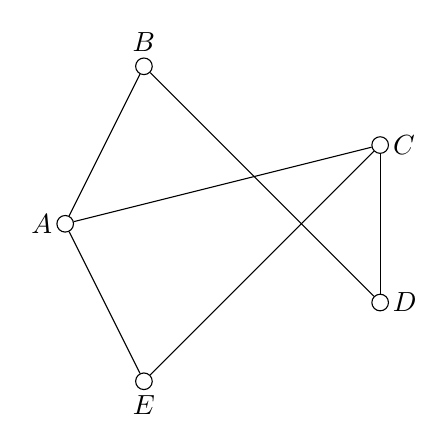
\begin{tikzpicture}
        \tikzstyle{every node}=[draw, circle, fill=white,
            minimum size=6pt, inner sep=0pt]
            \draw (0,0) node (a) [label=left:$A$] {};
            \draw (1,2) node (b) [label=above:$B$] {};
            \draw (4,1) node (c) [label=right:$C$] {};
            \draw (4,-1) node (d) [label=right:$D$] {};
            \draw (1,-2) node (e) [label=below:$E$] {};

            \draw (a) to (b);
            \draw (a) to (c);
            \draw (a) to (e);
            \draw (b) to (d);
            \draw (c) to (d);
            \draw (c) to (e);
    \end{tikzpicture}
    \captionof{figure}{Граф авиарейсов}
\end{center}

Сразу видно, что из города $A$ можно долететь до города $D$ как с
одной пересадкой, так и с двумя. При этом пути, то есть
последовательности вершин, в которых каждые соседние вершины 
соединены ребром (или смежны), будут такими: $A-B-D$, $A-C-D$ или
$A-E-C-D$. На второй вопрос ответить немного сложнее: удалять по
очереди все ребра --- не лучшее решение, ведь граф может быть
большим. Гораздо удобнее найти цикл (то есть путь, первая и
последняя вершины которого совпадают), например, содержащий все
вершины. И действительно, такой цикл сразу находится: $A-B-D-C-E-A$.
Теперь можно заключить, что если мы удалим ребро из цикла, то
связность (возможность добраться из любого города до любого другого)
сохранится --- достаточно двигаться по оставшемуся от цикла пути. При
удалении ребра не из цикла связность тем более не нарушится.

\begin{task}
    На доске $3 \times 3$ в углах $a1, c1, a3, c3$ поставлены
    черные (снизу) и белые (сверху) кони. Можно ли их поменять местами,
    чтобы черные оказались внизу, а белые наверху? Какое минимальное
    число ходов потребуется? Можно ли сделать так, чтобы кони
    стояли в углах, а их цвета чередовались по кругу?
\end{task}

Ответить на первый вопрос достаточно просто --- можно предъявить
последовательность ходов, которая поменяет коней местами. Но
следующие вопросы не столь очевидны. Как доказать минимальность?
Как доказать, что нельзя поставить коней так, чтобы их цвета
чередовались? Здесь нам снова помогут графы.

Попробуем нарисовать граф ходов. Вершинами будут клетки на
доске, а ребра будут проведены так, что вершина соединена
с другой, если на доске из соответствующей клетки можно
попасть во вторую ходом коня. Если мы аккуратно нарисуем
такой граф, получится очень простая картинка:
\begin{center}
    \begin{tikzpicture}
        \tikzstyle{empty}=[draw, circle, fill=black,
            minimum size=1pt, inner sep=0pt]
        \tikzstyle{white}=[draw, circle, fill=white,
            minimum size=6pt, inner sep=0pt]
        \tikzstyle{black}=[draw, circle, fill=black,
            minimum size=6pt, inner sep=0pt]
        \node[black, label=below:a1] (a1) at (0, -3) {};
        \node[empty, label=right:b3] (b3) at (2, -2) {};
        \node[black, label=right:c1] (c1) at (3, 0) {};
        \node[empty, label=right:a2] (a2) at (2, 2) {};
        \node[white, label=above:c3] (c3) at (0, 3) {};
        \node[empty, label=left:b1] (b1) at (-2, 2) {};
        \node[white, label=left:a3] (a3) at (-3, 0) {};
        \node[empty, label=left:c2] (c2) at (-2, -2) {};
        \node[empty, label=above:b2] (b2) at (0, 0) {};

        \draw (a1) to (c2);
        \draw (c2) to (a3);
        \draw (a3) to (b1);
        \draw (b1) to (c3);
        \draw (c3) to (a2);
        \draw (a2) to (c1);
        \draw (c1) to (b3);
        \draw (b3) to (a1);

    \end{tikzpicture}
    \captionof{figure}{Граф передвижения коней по доске}
\end{center}
Теперь хорошо видно, как устроены возможные перемещения коней. Они
передвигаются по циклу, значит, для перемены цветов достаточно,
чтобы каждый конь прошел полоборота. Тогда потребуется 16 ходов.
При этом количество минимально, поскольку порядок коней друг
относительно друга по кругу не меняется при движении. То есть
конь с $a1$ должен обязательно прийти на поле $c3$. Для этого
потребуется как минимум 4 хода. Для остальных коней рассуждение
аналогично. Итого 16 ходов.

Остался последний вопрос --- можно ли сделать так, чтобы цвета
чередовались. Но с помощью графа и на этот вопрос ответить легко:
нельзя, потому что кони не могут <<обгонять>> друг друга.

\begin{task}[Семь мостов Кенигсберга]
    Можно ли совершить прогулку по Кенигсбергу, пройдя по каждому
    из мостов и вернувшись в исходную точку?
\end{task}
\begin{center}
    \includegraphics[width=10cm]{bridges-euler}
    \captionof{figure}{Схема мостов в Кенигсберге}
\end{center}

Это классический пример. Данная задача была решена Леонардом 
Эйлером и описана в его статье (рисунок взят как раз из нее).
Попробуем представить задачу в виде графа. Вершинами будут
части суши, а ребрами --- мосты. Получим следующую картинку:

\begin{center}
    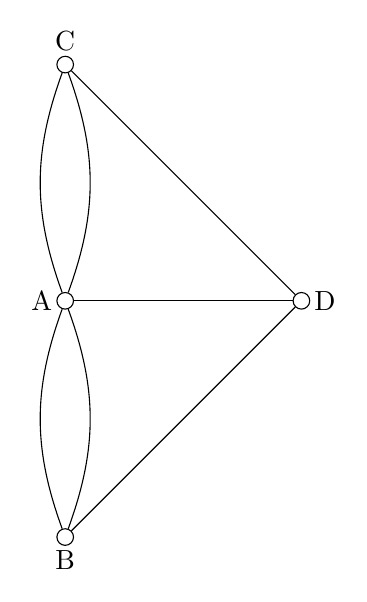
\begin{tikzpicture}
        \tikzstyle{vertex}=[draw, circle, fill=white,
            minimum size=6pt, inner sep=0pt]
        \node[vertex, label=left:A] (A) at (0, 0) {};
        \node[vertex, label=below:B] (B) at (0, -3) {};
        \node[vertex, label=above:C] (C) at (0, 3) {};
        \node[vertex, label=right:D] (D) at (3, 0) {};

        \draw (A) [bend left=20] to (B);
        \draw (A) [bend right=20] to (B);
        \draw (A) [bend left=20] to (C);
        \draw (A) [bend right=20] to (C);
        \draw (A) to (D);
        \draw (B) to (D);
        \draw (C) to (D);

    \end{tikzpicture}
    \captionof{figure}{Граф мостов в Кенигсберге}
\end{center}

Заметим, что здесь у нас между двумя вершинами может быть
несколько ребер (такие ребра называются кратными).
Нас интересует такой факт: существует ли в графе цикл,
содержащий все ребра и проходящий по каждому ребру ровно один
раз (такой цикл называется эйлеровым)? Легко заметить, что
такого цикла здесь нет. Действительно, пусть он есть.
Посмотрим на вершину $D$ и начнем прогулку из нее.
В какой-то момент мы должны вернуться. Заметим, что каждое
посещение вершины $D$ использует два новых ребра из нее. Но
степень вершины (количество выходящих из нее ребер) нечетна,
значит, закончить маршрут в ней мы не сможем. Получается,
таким образом прогуляться по Кенигсбергу не получилось бы.

\subsection{Простые результаты}

До сих пор мы разбирали частные примеры графов, которые
полностью заданы и даже представимы в виде простой картинки.
Часто же приходится работать с графами, о которых известно
мало (например, ничего). Чтобы разобраться с этим, рассмотрим
простой, но важный результат.

\begin{lemma}[О рукопожатиях]
    В любом графе сумма степеней вершин равна удвоенному числу
    ребер.
\end{lemma}
\begin{proof}
    Воспользуемся подсчетом двумя способами. С одной стороны
    мы имеем сумму степеней вершин. С другой --- мы можем
    каждую степень рассмотреть, как число ребер, выходящих
    из соответствующей вершины. Если мы просуммируем по всем
    вершинам (то есть сложим все степени) и возьмем во
    внимание, что каждое ребро выходит ровно из двух вершин,
    получим требуемое.
\end{proof}

Данная лемма имеет такое название, поскольку задачу (как и
многие другие задачи, связанные с графами) можно сформулировать
иначе. На встречу пришла компания людей. Все пары знакомых людей
пожали друг другу руки. Докажите, что удвоенное число рукопожатий
равно числу знакомых, сложенному по всем участникам встречи.
Отсюда получаем простое следствие: число участников, сделавших
нечетное количество рукопожатий, четно. В терминах графа:

\begin{corollary}
    В любом графе число вершин с нечетной степенью четно.
\end{corollary}

Рассмотрим еще одну простую задачу.

\begin{task}
    В графе на $2n+1$ вершинах степень каждой вершины не меньше $n$.
    Докажите, что граф связен.
\end{task}

Мы докажем более сильное утверждение: расстояние (длина кратчайшего пути
с концами в данных вершинах) между любыми двумя
вершинами данного графа не превосходит 2. Для этого возьмем произвольные
две вершины $v$ и $u$. Если они соединены ребром, то утверждение
выполнено. В противном случае посмотрим на оставшиеся $2n-1$ вершины. Из
них найдем $n$ вершин, соединенных с $v$ и $n$ вершин, соединенных с $u$.
Среди них существует вершина, соединенная как с $v$, так и с $u$. Из
произвольности выбора вершин следует утверждение задачи.

\begin{center}
    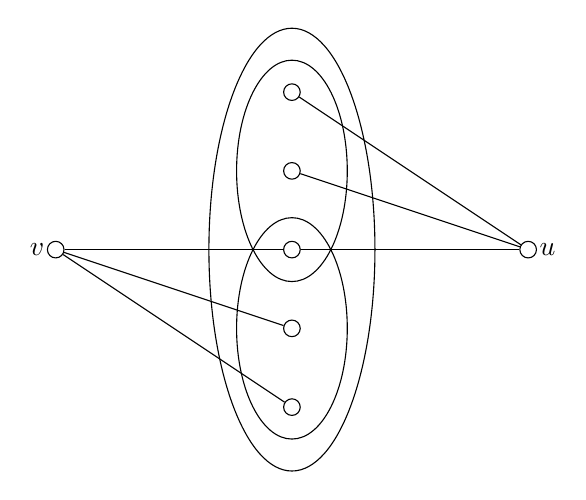
\begin{tikzpicture}
        \tikzstyle{vertex}=[draw, circle, fill=white,
            minimum size=6pt, inner sep=0pt]

        \node[vertex, label=left:$v$] (v) at (-3, 0) {};
        \node[vertex, label=right:$u$] (u) at (3, 0) {};
	
	\draw (0, 0) ellipse (30pt and 80pt);
	\draw (0, -1) ellipse (20pt and 40pt);
	\draw (0, 1) ellipse (20pt and 40pt);

        \node[vertex] (w1) at (0, 0) {};
        \node[vertex] (w2) at (0, -2) {};
        \node[vertex] (w3) at (0, -1) {};
        \node[vertex] (w4) at (0, 2) {};
        \node[vertex] (w5) at (0, 1) {};

        \draw (v) to (w1);
	\draw (v) to (w2);
	\draw (v) to (w3);
	\draw (u) to (w1);
	\draw (u) to (w4);
	\draw (u) to (w5);
    \end{tikzpicture}
    \captionof{figure}{Граф из задачи 10}
\end{center}

Часто бывает полезным найти вершину или, например, путь, обладающий
некоторым свойством: вершину с наибольшей (наименьшей) степенью, самый
длинный (короткий) путь и так далее. Рассмотрим задачу, в которой это
используется.

\begin{task}
    Докажите, что в связном графе можно удалить вершину и выходящие из
    нее ребра так, что оставшийся граф будет также связен.
\end{task}

Рассмотрим произвольную вершину $v$. Для нее выберем такую вершину $u$,
что расстояние от $v$ до $u$ максимально. Удалим вершину $u$ и покажем,
что оставшийся граф не потерял связность. Заметим, что для любой вершины
$w$ в исходном графе кратчайший путь до $v$ не мог проходить через вершину
$u$ (поскольку $u$ --- наиболее удаленная от $v$ вершина). Значит, всякая
вершина $w$ в исходном графе была соединена путем, не проходящим через
$u$, с вершиной $v$. Но тогда $w$ будет в новом графе соединена с $v$
этим же путем. В силу произвольности $w$ весь граф является связным.

Снова надо соблюдать аккуратность в рассуждениях по индукции. Приведем
простой пример ошибки в рассуждениях.

\begin{example}
    Докажем, что если в графе нет изолированных вершин, он связен.
\end{example}

Граф из одной вершины связен. Даже граф из двух вершин связен.
Возьмем граф из произвольный граф на $n$ вершинах, в котором
нет изолированных вершин. По предположению индукции он связен.
Добавляем новую вершину --- поскольку она не изолирована, есть
ребро, соединяющее ее с остальным графом. Значит, и весь граф
связен.

Ошибка здесь достаточно проста: таким способом мы можем получить
не все графы. Корректнее брать произвольный граф, выбирать в нем
вершину, удалять ее и применять предположение индукции к оставшемуся
графу. Далее необходимо вернуть вершину и закончить рассуждение.
